% Copyright (c) 2014,2016 Casper Ti. Vect
 
\chapter{绪论}

	现金法定货币,交易凭据及交易数据库存在着一些缺点。如现金很难杜绝假钞的横行,交易凭据有着伪造的可能,在交易数据库中信息不一致,数据库被DDOS攻击,交易数据被窜改,数据库损毁,都是在传统交易过程中曾出现过的窘境。

	于2009年加密货币 - 比特币\supercite{bitcoinpaper}的问世,以密码学、网络学与货币银行学为基础创建了新一代的网络货币。各式网络货币中又以比特币最为广泛使用,其防堵被窜改、公开交易数据查看、使⽤者具匿名性、⾃动运作不须⼈为运营等等多项特性深受现今用户喜爱。至今区块链技术已成为IBM、摩根大通、微软、谷歌与英特尔等重点开发项目,被视为改善银行运作效率、降低运营成本、提升信息安全、创建公开数据的最佳方法。为解决现金、收益及交易数据库存在之问题,本文采用以区块链为基础的加密货币比特币为基础,进行商业化收银系统开发。不仅是基于⽐特币算法稳定、交易公开透明、不可被窜改等特性,同时本论⽂更加⼊监督标签,促使在匿名交易转为部分实名交易之过程中,监管部⾨能有更好的新兴货币技术的提升,亦可创建自动化的税务审查机制,大幅降低人事成本,进而实现提升交易系统信息之可靠度与其稳定性。

	\section{选题背景}

		追溯着加密货币市场的演进,于2009年时,比特币并非第一个加密货币,在比特币之前已经有着很多类似的加密货币开发实验,但是一直无法做出一个稳定点对点式的电子现金系统,关于其制作瓶颈之部分将于后段章节阐述。在比特币稳定发展之后,有着许多对比特币有兴趣的研究者,以稳定的比特币系统为基础修改了许多基本的协议。于2011年相继创造出了货币,将其称之为⼭寨币。山寨币早期较为著名包括有莱特币(Litecoin,LTC)\supercite{litecoin}、狗币(Dogecoin,DOGE)\supercite{dogecoin}、域名币(Namecoin,NMC)\supercite{namecoin},于2014年也有人认为比特币挖矿使用到了大量的哈希运算,这样的大量运算也浪费了许多的社会资源,进而开发出较具意义的工作量证明挖矿算法,其中较为著名的如素数币(Primecoin,XPM)\supercite{primecoin}。 于2015年底也诞生了现在最为著名的以太坊经典(Ethereum Classic,ETC)\supercite{ethereumclassic}、以太坊(Ethereum,ETH)\supercite{ethereum},以太坊最重⼤突破设计在于将编程语⾔虚拟机移植到了区块链架构上,这使得区块链技术不再仅止于点对点的电⼦现⾦系统,也创造出了属于以太坊的编程语言Solidity\supercite{solidity},使以太坊在虚拟机(Ethereum Virtual Machine,EVM)\supercite{Ethereum:Asecuredecentralisedgeneralisedtransactionledger}中可以使⽤Solidity 创建智能合约,合约可以建构去中心化的应用程序,如去中心化的交易所,将交易所去中心化可以有效的防治DDOS攻击 \supercite{Bitcoin:Economicstechnologyandgovernance},降低交易所因为黑客攻击而倒闭的可能性。
		

		\subsection{加密货币市场}

		加密货币中最具代表性的是比特币,但除了比特币之外也存在许多模仿比特币的加密货币,有的是为其利益,有的是鉴于比特币的各种不足,进而希望借由其他货币改善⽐特币不够完美之处。加密货币市场中有成千上万种的加密货币,其中较广为人知的加密货币会在Cryptocurrency Market Capitalizations\supercite{CryptocurrencyMarketCapitalizations}的排行榜中出现,截至2018年2月8日该排行榜已经收入了1510种加密货币。在Cryptocurrency Market Capitalizations统计的数据当中,可知整体的加密货币市场,如图\ref{TotalMarketCapitalization}所示,于2018年1月7日创下了历史新高,加密货币市场的总市值也高达了829,579,000,000美金,相当于五兆人民币的总市值。

		\begin{figure}[!htbp]
			\centering
			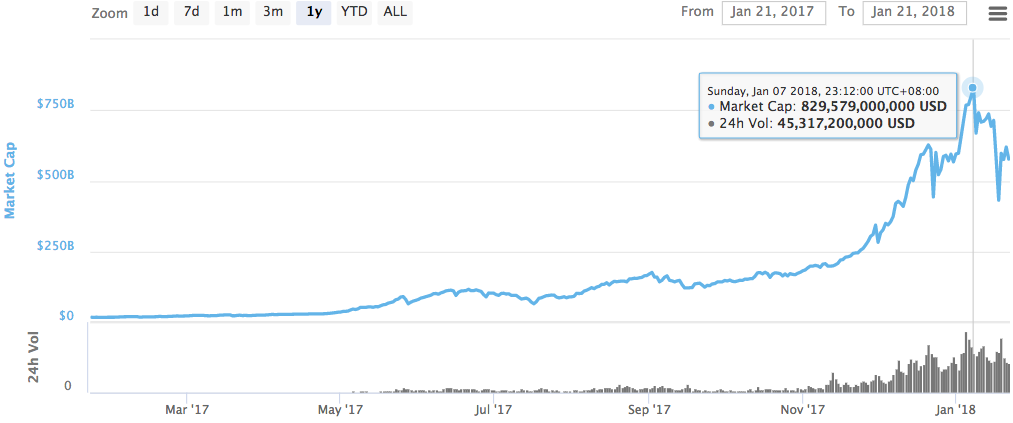
\includegraphics[width = 1\textwidth]{TotalMarketCapitalization.png}
			\caption{2017年1月21日到2018年1月21日期间加密货币总市值走势图\supercite{CryptocurrencyMarketCapitalizations}}\label{TotalMarketCapitalization}
		\end{figure}

		经由Cryptocurrency Market Capitalizations数据显示,整体加密货币市场自2013年起已经高达150亿美金,2014年与2015年间总市值减少到近乎2013年的一半。针对比特币的价格波动,论文"Have the security flaws surrounding Bitcoin effected the currency's value?."
		\supercite{HavethesecurityflawssurroundingBITCOINeffectedthecurrencysvalue?}
		作出详尽的市场调研,致力于探讨在各个比特币市场大事件中对比特币价格的波动影响,针对影响的程度该论文给出影响指数,当中影响最为严重的是于2014年2月发生的日本交易所Mt.Gox倒闭事件,因为早期的加密货币市场中无完善的法律规范,各国对加密货币的接受度有所不同,日本对金融科技的接受度相较于较为开放的情况下成立了全世界第一家比特币交易所Mt.Gox,也因为交易所不够普及,使得大部分的加密货币交易都集中在Mt.Gox交易所中,使Mt.Gox 倒闭事件成为震荡市场价格重⼤因⼦之⼀,也造成2014与2015年的加密货币市场低迷。而在2017年,比特币又以2016年总市值之35倍的姿态攀上新高点,主要是因为美国最大的期权交易中心芝加哥期权交易所(Chicago Board Options Exchange, CBOE)于2017年12月10日宣布支持比特币期货交易,此举将比特币价格推升到20,000美金的历史新高,图\ref{Thetotalmarketcapitalization}为2013年至2018年间比特币总市值K线图。

			\begin{figure}[!htbp]
				\centering
				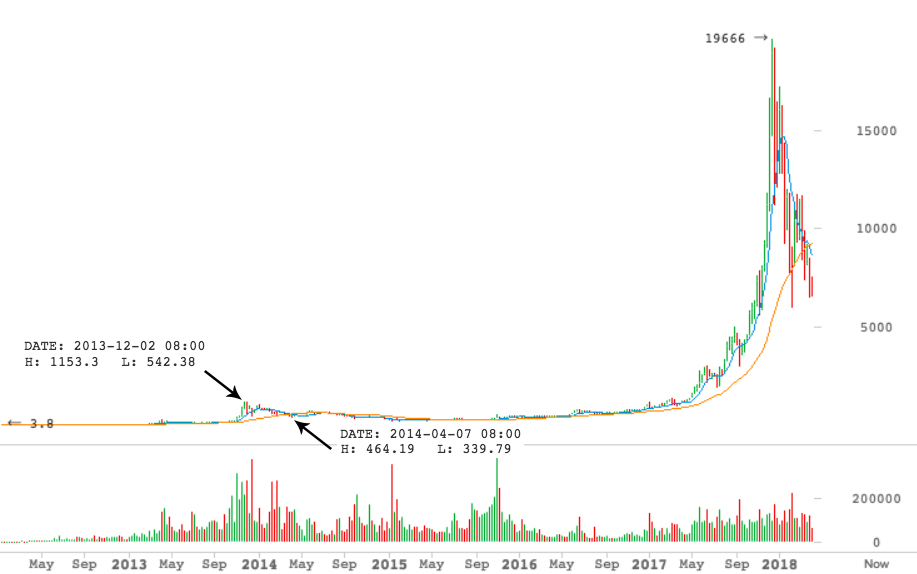
\includegraphics[width = 1\textwidth]{Thetotalmarketcapitalization.jpg}
				\caption{2013年至2018年间比特币总市值K线图\supercite{CryptocurrencyMarketCapitalizations}}\label{Thetotalmarketcapitalization}
			\end{figure}
		

			\subsection{加密货币的优势}
			于2009年Satoshi Nakamoto发布了比特币系统,成为全世界第一个加密货币的雏形。其透明的交易信息、区块链交易数据无法修改和删除、匿名与⾃治系统等特性,促使区块链技术冲破现存传统中⼼化之⾦融机构技术上的籓篱。以下将逐一说明加密货币的七项优点,分别为区块链结算系统不间断的运行、远距离支付、货币为用户持有、开放和透明的交易信息、区块链交易数据无法修改和删除、交易匿名性以及自治性系统。

				第一,区块链结算系统不间断的运行。基于区块链技术与点对点网络的架构,以比特币为例,自2009年至今,所有的比特币交易事件皆会存储在比特币区块链当中,区块链既无法删除也无法修改,比特币区块链会以点对点网络的方式存储在比特币网络中的全节点\supercite{YouReallyShouldRunaBitcoinFullNode:HeresWhy},目前比特币网络中的全节点高达11147个。与传统中心化的银行数据库相比,可能会因为银行的服务器维护,导致交易无法顺利进行,甚至可能有黑客的入侵导致银行或是个人资产有重大的损失。点对点网络提供稳定的数据库元数据,不会因为数据库的停机而无法继续使用,实现其24小时不间断之运作。
				
				第二,基于点对点网络架构完成远距离支付。于跨国汇款从美国转帐至中国一百万美金的场景中,需要经过的手续较为繁琐,资金有可能需要经过多个国家才可以抵达目的地,在经过各个国家的过程中,需要支付各国的手续费,也需要等待各个国家办理该业务的时间,即使当资金顺利抵达了目的地银行,目的地银行也需要花将近三至五日的工作日确认该笔金额的来源。届时领款人亦需要前往银行核实完整的身份验证、解释资金用途,才得以领取这笔跨国资金。比特币系统当中,有着24小时不间断运作的优点,也因为点对点网络架构,使得比特币无需经由传统金融机构繁琐的步骤完成国际汇款,于比特币系统中无系统壅塞的情况下,平均10分钟即可入帐,实现其短时间内即可完成远距离支付之运作。

				第三,加密货币为用户持有。传统的金融体系中,资金的存储、流动往往需要经过银行,用户将所有的资产存入银行,拿到的是一串数字的银行余额,银行是一个中心化的机构,有着最高的权利。中央社的新闻\supercite{Bankguardsstolen}指出,台湾各地于2017年接连于土地银行、日盛银行、彰化银行、京城银行、兆丰银行皆传出银行行员监守自盗的行为,总金额高达一亿三千万新台币。在比特币系统中,比特币有如金币般存放在个人的比特币地址当中,用户为真实持有着货币,即使是比特币系统亦无权利动用该笔比特币资产,唯有比特币地址的私钥持有者,才可以转移该笔比特币地址中的比特币资产。

				第四,公开的交易信息。基于区块链架构,所有的交易信息皆以公开的方式存储于区块链中,并且可信任与方便的取得元数据,以下将针对可信任与元数据进行探讨。
				\begin{enumerate}
					\item 可信任:在公有链的基本架构上,所有的交易记录都是公开透明的存储在区块链当中,比特币网络的用户都可以查看该笔交易,所有人都可以检查每个交易记录的正确性,公开的交易信息亦提升交易数据之可信性。
					\item 元数据:除了以区块链技术为基础建构出可信任的系统之外,开放和透明的特性让更多的开发商或新公司得以更容易获得交易的元数据。毕竟,在传统金融体系中,所有交易记录均由中央金融机构存储,从中央金融机构提取原始交易信息并不容易,区块链的开放性和透明性促使金融公司降低了获取原始数据努力的门槛。公司或学者可以透过元数据制定出可视化的开发计划,甚至可以运用大量数据来分析前所未达的新价值观点。
				\end{enumerate}

				第五,区块链交易数据无法修改和删除。在区块链结构中,通过严格验证的所有信息都记录在区块链中,且用户及系统平台都不赋与删除及修改之权限。根据区块链的特点,旧区块的哈希值在连接区块链的过程中,旧区块的哈希值会被存储在新区块。只要区块中的值被修改,即使仅有1 bit的变化,也会产出完全不同的哈希值,这也就是所谓的雪崩效应(Avalanche effect)\supercite{Theuseofbentsequencestoachievehigher-orderstrictavalanchecriterioninS-boxdesign}。由于上述结构特性,区块链中所有的信息都会被系统纪录且都不会被改变,倘若区块中记载的比特币交易在其中一个比特币全节点验证的结果被窜改,则该区块将不被比特币系统接受。因此,所有已经存储在区块链中的交易记录将不能被修改和删除,进而实现其架构安全之稳固。

				第六,区块链系统中所有的用户皆为匿名。现今社会中,个人信息保护已成为企业最重要的课题。在区块链系统中创建的所有帐户都不会与真实世界中的实体创建直接关联,也因为没直接关联所以创建匿名。区块链系统中的所有帐户都是由匿名个体创建,匿名的设计可以有效保护消费者的隐私。然而,VISA交易与比特币系统截然不同,在使用VISA支付系统前,用户必须向VISA公司的主机提交大量个人信息,这可能会产生个人信息泄露的风险。在区块链技术中,其匿名之特性可以有效地避免这个问题。

				第七,自治系统。在区块链系统中,区块链的运作依赖于一些算法,包括共识算法。因此,在这种自治系统中,没有人(例如节点或矿工)可以直接改变系统运作的规则。如果在比特币系统中发现需要更正的严重错误,可以使用比特币改进提案(Bitcoin Improvement Proposals,BIP)\supercite{BitcoinImprovementProposals}升级比特币系统。 在实施比特币改进提案之前,提议的比特币改进提案需要得到比特币系统中超过一定数量的矿工算力支持。由于这种以投票机制升级系统的门槛相当高,使得区块链系统通常不会有大的变化,因为变化不⼤也突显其相对稳定性。

			\subsection{加密货币的劣势}
			在区块链技术中,有着三项瓶颈,分别为每秒处理的交易量(Transactions Per Second,TPS)仅为7笔的限制、洗钱防治困难、低可扩展性,以下将逐一探讨。

				第一,每秒处理的交易量上限仅为7笔。图\ref{TPS}为国际上较为广泛使用的⽀付系统之每秒⽀持交易量⽐较图,以VISA为例,其以公司中心化运营的方式可以支持高达每秒2,000笔交易。但是以区块链技术为基础的比特币最大能够接受的每秒处理交易量仅为7笔。一般认为只要提升区块大小的限制,就可以提升每秒处理的交易量。提升每秒处理交易量的同时将产生下述的两项问题,分别为区块链成长速度过快造成节点崩溃以及区块同步延迟造成区块链分岔:

					\begin{figure}[!htbp]
						\centering
						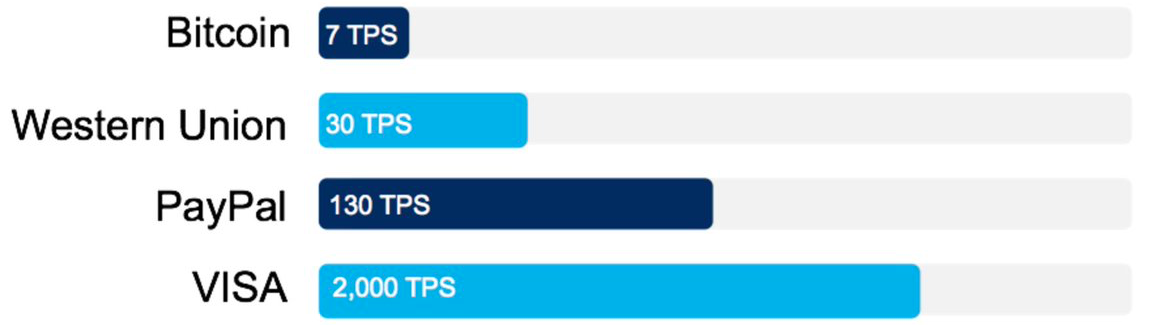
\includegraphics[width = .6\textwidth]{TPS.png}
						\caption{Bitcoin、Western Union\supercite{WesternUnion}、PayPal\supercite{PayPal}以及VISA每秒支持交易量比较图\supercite{digibyte}}\label{TPS}
					\end{figure}

					\begin{figure}[!htbp]
						\centering
						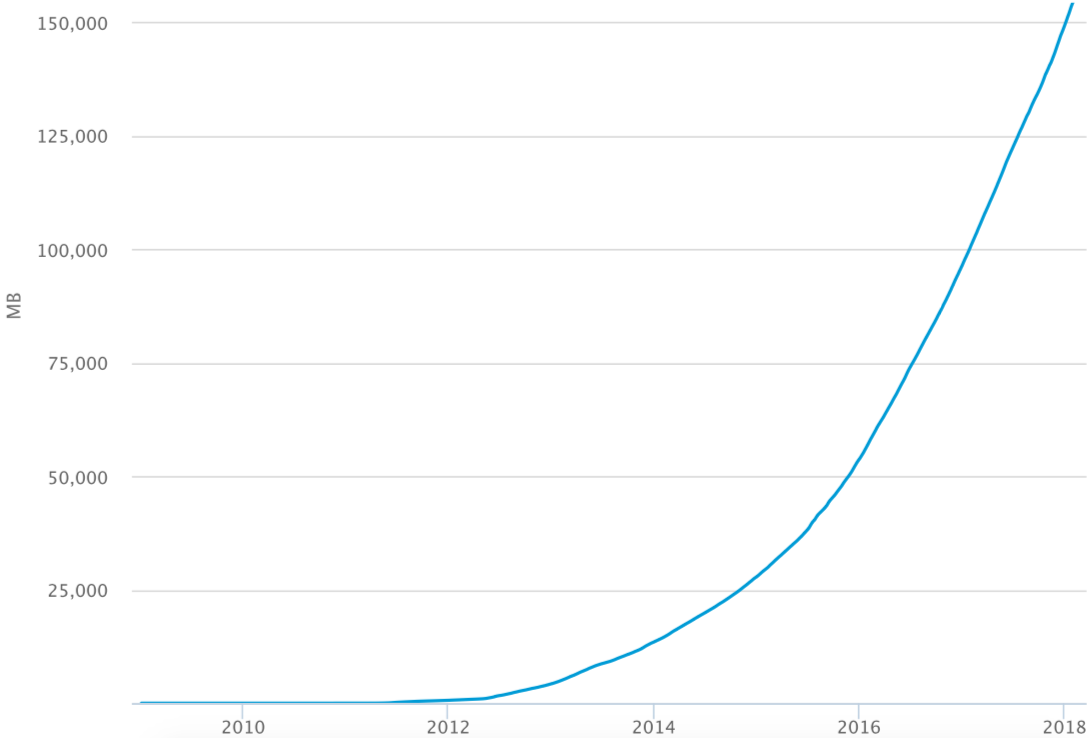
\includegraphics[width = .8\textwidth]{blockchainsize.png}
						\caption{比特币区块链成长走势图\supercite{blockchainsize}}\label{blockchainsize}
					\end{figure}


					\begin{enumerate}
						\item 区块链成⾧速度过快造成节点崩溃。区块链成长速度过快会造成比特币全节点不堪负荷:从2009年至今的比特币区块链大小已达到188.89 GB,这样的成长速度因为比特币区块大小的最大值被设置为1 MB。图\ref{blockchainsize}为过去比特区块链大小,图中可以发现,于2016年开始,比特币区块链的成长速度为一直线,这表示着比特币网络中持续维持在供不应求的状况。为解决比特币每秒⽀持交易量上限的窘迫,现今对⽐特币的每秒处理交易量有许多优化的⽅案,其中包括解除比特币区块大小1 MB的限制。在一个区块上限为1 MB的限制下,满载的比特币系统中,比特币区块链平均每十分钟会增1 MB,每小时会增加6 MB,每天会增加144 MB,每月会增加4.2 GB,每年会增加高达50 GB,要达到1 TB的区块链大小还需要8年,在8年后的未来存储1 TB的数据量应该不会有太大的负担。倘若解除1 MB的区块限制,在系统的每秒处理交易量看似可以接受更多的交易成倍成长,面临1 TB的比特币区块链数据会在更短的时间内出现,倘若存储区块链的成本超过了摩尔定律的成长曲线,会进一步造成用户自愿成为比特币全节点的意愿度降低,使得比特币网络的全节点数变少,导致比特币点对点网络逐渐转向中心化网络发展,失去一开始点对点网络的意义。

						\item 造成区块链最新区块同步延迟而使区块链分岔。对于区块链的区块同步延迟同时也会造成比特币网络的影响,J. Göbel于"Increased block size and Bitcoin blockchain dynamics"\supercite{TelecommunicationNetworksandApplicationsConferenceITNAC201727thInternational}有着详细的研究,在上修区块大小上限的议题上,用户因系统占用量提高,⾃愿成为⽐特币全节点意愿度下降,此举可能对⽐特币点对点网络建构出的区块链同步上造成延迟,在11147个比特币全节点当中,平均每十分钟会有矿工于其中一个全节点生成一个最新的区块,该最新的区块会以点对点网络协议同步到其他11146个节点上。在比特币系统中,长年来的过程经验可以发现在矿工生成1 MB的区块后同步到全网节点可以在创造下一个区块之前完成。倘若将区块大小修改为2 MB或是更大,会使得比特币全节点的最新区块同步延迟现象更加明显,同步延迟会使得区块链分岔,造成11147个比特币全节点的信息不一致,近一步造成整个比特币点对点网络崩溃。
					\end{enumerate}
					

				第二,洗钱防治困难。匿名性为比特币系统一大特色,比特币的地址生成的熵是256 bits,乱数是在$2^{256}$的组态空间中随机选取,这样的地址与现实生活中的身份并无任何关联,使得黑市交易、洗钱防治变的困难,甚至有更为前沿的加密货币Monero\supercite{noether2014monero}导入了环签章(Ring Signature)\supercite{Thresholdringsignaturesandapplicationstoad-hocgroups}算法、Zcash\supercite{zhong2002faster}导入零知识证明算法\supercite{Zero-KnowledgeProofsofIdentity},使得原本公开透明的区块链,变得无法查看,进而造成加密货币在洗钱防治上更加的困难。2017年由Thibault de Balthasar and Julio Hernandez-Castro 所提出的论文"An Analysis of Bitcoin Laundry Services."\supercite{AnAnalysisofBitcoinLaundryServices},致⼒探究⽐特币匿名交易下的资⾦流动模型,试图以机械学习的方法找出比特币洗钱模型作为洗钱的工具,图\ref{Darklaunderworkflow}为该论文针对黑市交易中的洗钱服务运营商Darklaunder进行洗钱机
					\begin{figure}[!htbp]
						\centering
						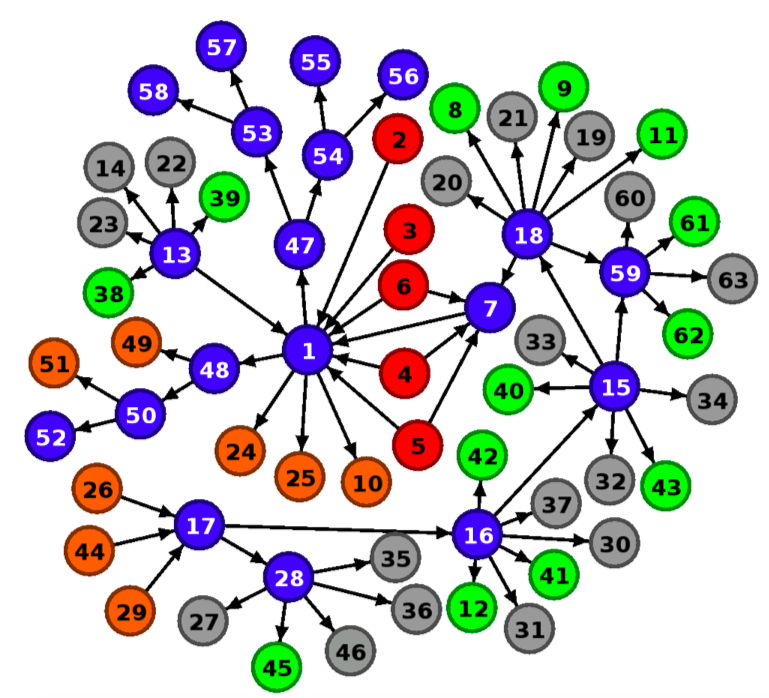
\includegraphics[width = .6\textwidth]{Darklaunderworkflow.png}
						\caption{Darklaunder 洗钱模型\supercite{AnAnalysisofBitcoinLaundryServices}}\label{Darklaunderworkflow}
					\end{figure}

				第三,低可扩展性。区块链架构为了防止各式的攻击,所以在架构订定以及接口设计都有着严谨的规范。以下将阐述造成比特币低可扩展性的原因:

					\begin{enumerate}

						\item 修改比特币协议制作添加外部信息的区块链:比特币区块链技术是一个严谨的架构,倘若要创造可以支持外部信息的结构需要重新创造全新的加密货币,大部分的加密货币不支持外部输入,由于外部的信息输⼊无法保证其信息的正确性,近一步造成垃圾进垃圾出(Garbage In, Garbage Out,GIGO)的问题,倘若错误的信息存储在无法删除、修改的区块链下,只是强化该笔错误信息的错误。如食品履历区块链,致力于将食品生产到超市的过程逐一记录在区块链上,但如果一开始在输入信息时,无法保证其信息之正确性,则该食品履历区块链则毫无意义,错误的信息内容甚至可能使该错误被强化。

						\item 于区块头或交易信息添加外部信息:比特币区块链上,可以添加一些信息于区块上,该信息会永久保存于区块链上,除了在区块上添加信息,在比特币单笔交易信息上,亦可填写一些私人信息,但这样的空间大小有限,且现今的比特币价格日趋上涨,比特币交易手续费是以单笔交易大小计算,这将使得在交易中添加些个人信息变得更加昂贵。

					\end{enumerate}

				在比特币系统中,其区块链仅用于记录交易记录,不能扩展更多功能和应用程序。有很多开发者希望将比特币系统扩展到智能合约等其他应用程序。但是,后来发现改变原始比特币系统框架是具有挑战性的工作。因此,全球第二大加密货币以太坊(Ethereum,ETH)的作者Vitalik选择了创建了以太坊虚拟机(Ethereum Virtual Machine,EVM),而非改变原始的比特币系统框架。以太坊虚拟机所创建的智能合约可以在统一的以太坊平台上运行,而以太坊也借此突破了比特币之技术瓶颈。
	
	\subsection{国际情势分析}
	\begin{table}[!htbp]
		\centering
		\caption{各国政府对比特币态度统整表}
		\label{world}
		\begin{tabular}{@{}|l|l|c|c|l|@{}}
		\toprule
		\multicolumn{1}{|c|}{\multirow{2}{*}{序号}} & \multicolumn{1}{c|}{\multirow{2}{*}{国家}} & \multicolumn{2}{c|}{接纳} & \multicolumn{1}{c|}{\multirow{2}{*}{禁止}} \\ \cmidrule(lr){3-4}
		\multicolumn{1}{|c|}{} & \multicolumn{1}{c|}{} & 欢迎/放任 & 监管 & \multicolumn{1}{c|}{} \\ \midrule
		1 & 伊朗 & \begin{tabular}[c]{@{}c@{}}监管得当欢迎\\ 比特币发展\end{tabular} &  &  \\ \midrule
		2 & 以色列 & \begin{tabular}[c]{@{}c@{}}欢迎:欲发展\\ 国际ICO中心\end{tabular} &  &  \\ \midrule
		3 & 法国 & \begin{tabular}[c]{@{}c@{}}放任:与实体\\ 经济无关\end{tabular} &  &  \\ \midrule
		4 & 美国 & 暂不构成威胁 &  &  \\ \midrule
		5 & 新加坡 & \begin{tabular}[c]{@{}c@{}}不监管但注意\\ 周边活动\end{tabular} &  &  \\ \midrule
		6 & \begin{tabular}[c]{@{}l@{}}沙特阿拉\\ 伯王国\end{tabular} & \begin{tabular}[c]{@{}c@{}}加密货币尚未\\ 成熟,不监管\end{tabular} &  &  \\ \midrule
		7 & 乌克兰 & 不属于货币 &  &  \\ \midrule
		8 & 韩国 &  & \begin{tabular}[c]{@{}c@{}}很快将监管\\ 交易所\end{tabular} &  \\ \midrule
		9 & 菲律宾 &  & 计划监管ICO &  \\ \midrule
		10 & 英国 &  & 考虑监管 &  \\ \midrule
		11 & 马来西亚 & \multicolumn{1}{l|}{} & 范式监管框架 & \multicolumn{1}{c|}{} \\ \midrule
		12 & 俄罗斯 & \multicolumn{1}{l|}{} & \begin{tabular}[c]{@{}c@{}}2018年7月前\\ 完成立法\end{tabular} & \multicolumn{1}{c|}{} \\ \midrule
		13 & 日本 & \multicolumn{1}{l|}{} & \begin{tabular}[c]{@{}c@{}}任命加密货币\\ 监察长\end{tabular} & \multicolumn{1}{c|}{} \\ \midrule
		14 & 香港 & \multicolumn{1}{l|}{} & ICO须受法规监管 & \multicolumn{1}{c|}{} \\ \midrule
		15 & 津巴布韦 & \multicolumn{1}{l|}{} &  & \multicolumn{1}{c|}{定法前,属非法} \\ \midrule
		16 & 摩洛哥 & \multicolumn{1}{l|}{} &  & \multicolumn{1}{c|}{禁止加密货币交易} \\ \midrule
		17 & 印尼 & \multicolumn{1}{l|}{} &  & \multicolumn{1}{c|}{\begin{tabular}[c]{@{}c@{}}2018年前\\ 全面禁止\end{tabular}} \\ \midrule
		18 & 中国 & \multicolumn{1}{l|}{} &  & \multicolumn{1}{c|}{禁止加密货币} \\ \bottomrule
		\end{tabular}
		\end{table}
	
	比特币是一种全新的价值交换的媒介,因为区块链技术相当新颖,在各个国家所秉持的态度皆有所不同,大致可将各个国家对比特币的政策分为两大类,分别为接纳与禁止;在接纳加密货币的分类当中又分为欢迎、放任以及监管。

	在欢迎、放任的政策下的国家包括伊朗、以色列、法国、美国、沙特阿拉伯王国、乌克兰以及新加坡,上述国家政策上皆已抱持着开放且不监管的方式接纳加密货币,这些国家认为加密货币对于国家金融科技的发展具有前景;在分类于接纳但是实施监管的国家中,包括韩国、菲律宾、英国、马来西亚、俄罗斯、日本以及香港地区皆认为加密货币技术可能存在的高风险,且针对加密货币的洗钱防制以及非法集资进行严格管理,也进一步制定相关的法律,使得国家可以应对新型加密货币的纠纷;在禁止加密货币的分类中包括津巴布韦、摩洛哥、印尼以及中国,这些国家认为比特币是一个非法的货币,因为涉及到洗钱问题、难以实施外汇管制。但是对于区块链技术层面上之探讨,在所有国家中都是以蓬勃发展的正面态度看待。上述各国政府对⽐特币态度如表\ref{world}:

		

	\section{研究目标与内容}
	比特币在各个国家的蓬勃发展且应用在相当多的领域,应用的领域包括交易所、去中心化交易所、兑币所、游戏点数、网络购物、资产的保存、募资以及远距离支付,甚至是各国的银行和金融机构都逐步投入人力及资金研究区块链相关技术,甚至是订定各国相关的法律。在比特币资产的流动上存在着许多的问题,第一,比特币的帐户是由乱数产生器生成,该比特币帐户与在现实生活中的用户并无直接关联,使得比特币洗钱变更加盛行。第二,现今的比特币交易皆为匿名对匿名支付,并无正式的交易凭据开立,使得消费者在购物后,倘若商品存在问题,无法得到法律上的保障。第三,因为比特币是匿名支付给匿名的交易,使得政府无法从交易行为中进一步课征税收,滞碍国家经济发展。

	本文将解决上述三项问题,设计与实现一个比特币的实时交易监督系统达到下列几点目标:

		\begin{enumerate}
			\item 导入匿名顾客支付给实名商家的交易模型到加密货币交易系统。
			\item 设计与实现在加密货币交易中匿名顾客支付给实名商家的交易监督系统。
			\item 于政府端导入多重签章算法,使比特币的实时交易监督系统比透过 Green Address 机构验证更加快速。
			\item 利用多重签章算法的机制可以让商家预防比特币双重支付的攻击。
			\item 商家和商品信息管理⼦系统让商家可进行库存管理及商家商品管理。
			\item 实现于加密货币交易中,消费者保持匿名同时也保障消费者权益。
			\item 透过对商家进行实名制,比特币的交易监督系统让政府主管机关可以有效获得税收。
		\end{enumerate}

	为实现上述目标,本文首先将详细探讨区块链技术的优势,借由深度了解区块链技术的优势可以取之优点,如区块链是一个不间断、不可窜改、去中心化、公开数据库、稳定的系统。第二,探讨区块链技术的劣势,区块链技术并非完美,存在着洗钱、逃漏税、无法保障消费者权益以及交易速度慢的问题,借由了解问题,并设计系统解决。第三,交易模型分析,透过交易模型分析探讨在现金、电子货币以及加密货币存在的交易模型,并在诸多交易模型中发现,匿名支付给实名的交易行为,可以保障消费者隐私,同时保障消费者权益,更使得政府可以对商家的营收进行查看。第四,系统设计,完成交易分析,并着⼿设计数据库模型。第五,系统详细设计与实现,利⽤Java 编程语⾔实现主系统以及三个⼦系统。第六,系统优化,引入比特币的多重签章算法,实现比特币的实时交易监督系统。第七,功能测试,测试以Java编写程序所有的功能是否能够完整运作。第八,性能测试,测试在未进行优化的系统与已经优化的系统两者之间性能的差异。


	\section{论文组织结构}
	在本节中将逐一说明本论文的组织结构共分为七章,分别为绪论、相关理论与技术、系统需求分析、系统概要设计、系统实现、系统测试以及总结与展望:

	第一章:简述区块链技术解决现有数据库存在的信息不一致、信息安全问题以及数据库损毁问题
	。说明在加密货币市场中不仅只是比特币,亦有许多新颖技术为特色的货币竞争。简要探讨区块链技术的优点,逐一探讨比特币的缺点及区块链技术瓶颈。最后于研究目标与内容当中,阐述本文的待解决问题以及解决方法。

	第二章:介绍比特币的发展,阐述比特币地址生成运用到的算法、生成过程以及多重签章算法。并详细说明区块链结构及所有字段变量与区块链相关的意义。

	第三章:首先对五种交易模型进行分析,进而得知匿名对实名的交易,既可以保障消费隐私且兼具保有消费者权益,并透过需求分析探讨本系统需构建的功能模块。

	第四章:概要设计比特币交易监督系统的架构,以及说明三个子系统的模块功能。设计本系统的数据库结构,设计ER实体联系模型 (Entity-relationship model),并阐述本系统的运作流程。最后则将多重签章算法引入本系统,使得本系统成为比特币的实时交易监督系统。

	第五章:详细设计商家和商品信息管理子系统、商家手持移动装置收款及交易子系统以及客户端行动支付和交易子系统的介面。

	第六章:透过功能测试逐一查看所有功能是否能够正常运行,经由性能测试分析原始系统与优化后的系统性能之间的差异。

	第七章:说明比特币区块链系统透过本文所提出之系统,可以达到保障消费者权益同时也兼顾保有顾客隐私,也使得政府可以透过该系统查看交易明细课征税收,而商家亦可对库存及产品进行管理,达到三赢的局面。
